\documentclass[a4paper, 12pt]{article}
\usepackage{graphicx}
\usepackage[T2A]{fontenc} 
\usepackage[utf8]{inputenc}
\usepackage[english, russian]{babel}
\usepackage{amsmath}
% \usepackage{xcolor}
% \usepackage{array}
\usepackage[left=2cm,right=2cm,top=1cm,bottom=0.5cm,bindingoffset=0cm]{geometry}
% \usepackage{float}
% \usepackage{wrapfig}
% \usepackage{tabularx}
\usepackage{nicematrix}
\usepackage{multirow}
\usepackage{multicol}
\pagestyle{empty}
\usepackage{graphicx}
\usepackage{amsfonts} 
\usepackage{stix}

\usepackage{nicefrac}
\usepackage[toc,page]{appendix}

\usepackage[babel=true]{microtype}
\usepackage{indentfirst}
\usepackage{tempora}  % Times for numbers in math mode
% \usepackage{newtxmath}  % Times in math mode

\usepackage[nottoc]{tocbibind}
\usepackage[toc,page]{appendix}
\usepackage{pdfpages}
\usepackage[rightcaption]{sidecap}
\usepackage{cite}
\usepackage[]{acronym}
% \usepackage[pdftex,scale={.8,.8}]{geometry}
% \usepackage[toc]{glossaries}
\usepackage[left,pagewise,modulo]{lineno}
\usepackage[pdftex,colorlinks=false,hidelinks,pdfstartview=FitV]{hyperref}
\usepackage[pagestyles,raggedright]{titlesec}
\usepackage[export]{adjustbox}
\usepackage{verbatim}
\usepackage{dirtytalk}
\usepackage{esvect}
% чтобы можно было делать больше матрицы
\makeatletter
\renewcommand*\env@matrix[1][\arraystretch]{%
  \edef\arraystretch{#1}%
  \hskip -\arraycolsep
  \let\@ifnextchar\new@ifnextchar
  \array{*\c@MaxMatrixCols c}}
\makeatother
 
\title{calc-sem-3-task-1}
\author{Давид Григорьев}
\date{November 2024}

\begin{document}


\begin{center}
	Министерство образования и науки Российской Федерации
	федеральное государственное автономное образовательное учреждение высшего образования
	\\
     {НАЦИОНАЛЬНЫЙ ИССЛЕДОВАТЕЛЬСКИЙ УНИВЕРСИТЕТ ИТМО}
    
    \vspace{2em}
    Факультет «Программной инженерии и компьютерной техники.»

    \vspace{10em}
    
    {\large Дополнительные главы математического анализа}\\
    
    \vspace{2em}
    
    {\large ИДЗ \textnumero2}
    \\
\end{center}
   

\vspace{20em}

\begin{flushright}
    \textbf{Выполнил} \\
    Григорьев Давид Владимирович\\
    Группа: P3215\\
    \textbf{Проверил}\\
    Попов Арсений Михайлович
    
\end{flushright}

\vspace{\fill}

\begin{center}
   Санкт-Петербург 2024
\end{center}


\newpage
\tableofcontents

\newpage

\pagenumbering{arabic}

\newpage

\section{Задание 1.}

Записать как двойной интеграл, сделать рисунок области и поменять порядок
интегрирования.
$$\int_{0}^{1}\, dy \int_{0}^{\sqrt{y}} f \, dx  + \int_{1}^{\sqrt{2}} \, dy\int_{0}^{\sqrt{2-y^2}} f \, dx $$

Чтобы записать как двойной интеграл, нужно определить область, по которой происходит интегрирование. Можно заметить, что по оси $Y$, два интеграла не пересекаются, значит, по свойству аддитивности, их можно будет объединить в один двойной интеграл по объединённой области.

\begin{figure}[h!t]
    \centering
    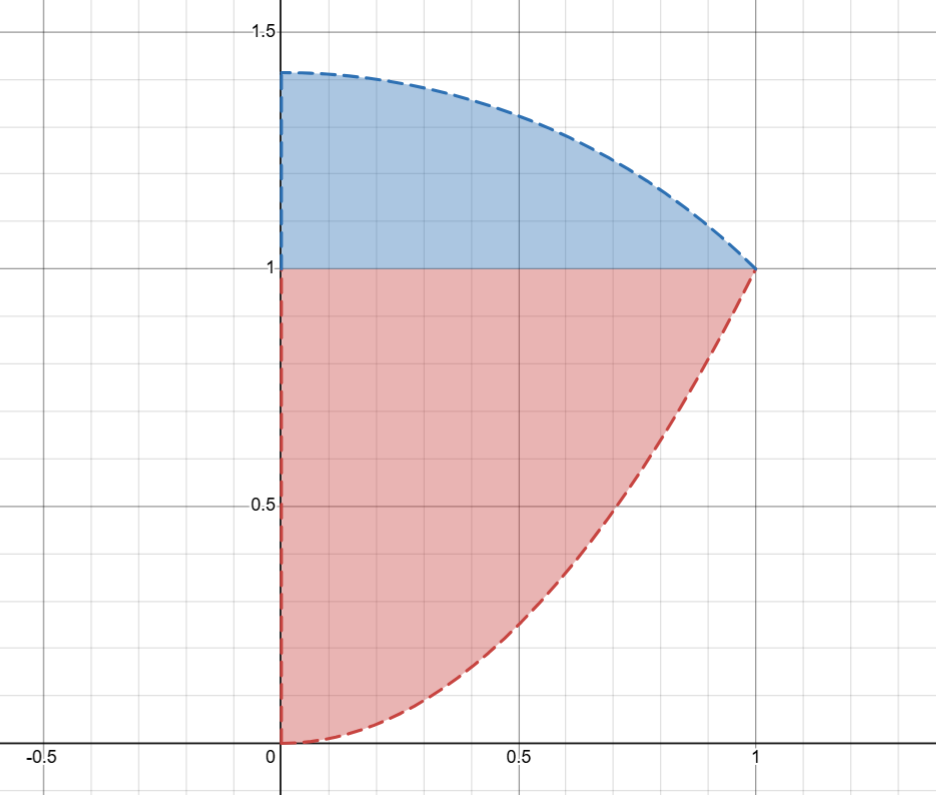
\includegraphics[width=0.3\linewidth]{Task1/Figure_shape.png}
    \caption{Задание 1. Область интегрирования.}
\end{figure}

Красным отмечена область левого интеграла, а синим - правого. Тогда можно записать двойной интеграл как
$$\int_{0}^{1}\, dy \int_{0}^{\sqrt{y}} f \, dx  + \int_{1}^{\sqrt{2}} \, dy\int_{0}^{\sqrt{2-y^2}} f \, dx = \iint\limits_D f dx\,dy $$

Где $D = \left\{0<x<\sqrt{y}\ \left\{0<y<1\right\}\right\} \cup \left\{0<x<\sqrt{2-y^{2}}\left\{1<y<\sqrt{2}\right\}\right\}$

Теперь попробуем поменять порядок интегрирования. Для этого нужно выразить $x$ через $y$ и наоборот.

Сначала выразим красную область. $x$ тут меняется внутри $(0,1)$, а $y$ найдем из неравенства.

$$0<x<\sqrt{y} \Rightarrow x^2 < y$$ 

И так как $x$ изначально был в $(0,1)$, то и $y$ будет идти до $1$. Тогда красная зона выражается так.

\begin{equation}
    x^2 < y < 1\left\{0 < x < 1\right\}
\end{equation}

Для синей области $x$ так же меняется внутри $(0,1)$. Этот $y$ тоже ограничен $1$, но уже снизу.

$$x<\sqrt{2-y^{2}} \Rightarrow x^2 < 2-y^2 \Rightarrow x^2-2 < -y^2 \Rightarrow y^2 < 2-x^2  \Rightarrow y < \sqrt{2-x^2}$$

\begin{equation}
    1 < y < \sqrt{2-x^2}\left\{0 < x < 1\right\}
\end{equation}

Теперь можно записывать это в виде интегралов, используя $(1)$ и $(2)$.

$$\int_{0}^{1}\, dy \int_{0}^{\sqrt{y}} f \, dx  + \int_{1}^{\sqrt{2}} \, dy\int_{0}^{\sqrt{2-y^2}} f \, dx = \int_{0}^{1}\, dx \int_{x^2}^{1} f \, dy  + \int_{0}^{1} \, dx\int_{1}^{\sqrt{2-x^2}} f \, dy $$

\href{https://www.desmos.com/Calculator/klqig4obxo}{Посмотреть задание в Desmos}

\newpage

\section{Задание 2.}

Область в $\mathbb{R}^2$ ограничена данными кривыми. Найти площадь с помощью двойного интеграла, выполнить рисунок.

$$ y^2 - 2y+ x^2 = 0, y^2 - 6y+x^2 = 0, y = \dfrac{x}{\sqrt{3}}, x = 0$$

Преобразуем данные равенства, чтобы было легче изобразить.

$$ \left(y^2 - 2y +1\right) - 1  + x^2 = 0, \left(y^2 - 2\cdot 3\cdot y + 3^2\right) -3^2 +x^2 = 0, y = \dfrac{x}{\sqrt{3}}, x = 0$$

$$ \left(y - 1\right)^2 + x^2 = 1^2, \left(y^2 - 3\right)^2 +x^2 = 3^2, y = \dfrac{x}{\sqrt{3}}, x = 0$$

Итого мы имеем два круга, один с радиусом $1$ и центром в $(0,1)$, и второй с радиусом $3$ и центром в $(0,3)$ и прямую с наклоном $\dfrac{1}{\sqrt{3}}$.

\begin{figure}[h!t]
    \centering
    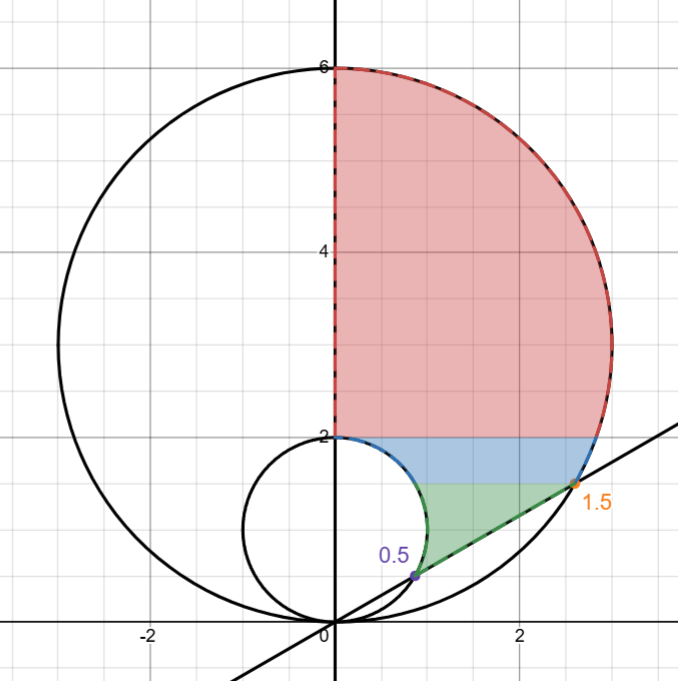
\includegraphics[width=0.3\linewidth]{Task2/Figure_shape.png}
    \caption{Задание 2. Области интегрирования \underline{\href{https://www.desmos.com/Calculator/spyqn3wlhu}{(Desmos)}}. }
\end{figure}

Нужный нам интеграл можно записать в следующем виде.

$$\iint\limits_{\text{Фигура}}1\,dx\, dy = \iint\limits_{\text{Красная}}1\,dx\, dy + \iint\limits_{\text{Синяя}}1\,dx\, dy + \iint\limits_{\text{Зеленая}}1\,dx\, dy = $$
$$= \int_2^6 \,dy \int_{0}^{\sqrt{9-\left(y-3\right)^{2}}}\,dx + \int_{1.5}^{2} \,dy \int_{\sqrt{1-\left(y-1\right)^{2}}}^{\sqrt{9-\left(y-3\right)^{2}}}\,dx + \int_{0.5}^{1.5}\int_{\sqrt{1-\left(y-1\right)^{2}}}^{y\sqrt{3}}\,dx = $$
$$=\int_2^6 \sqrt{9-\left(y-3\right)^{2}}\,dy + \int_{1.5}^{2} \sqrt{9-\left(y-3\right)^{2}} - \sqrt{1-\left(y-1\right)^{2}}\, dy + \int_{0.5}^{1.5} y\sqrt{3} - \sqrt{1-\left(y-1\right)^{2}}\, dy = $$
$$=\int_2^6 \sqrt{9-\left(y-3\right)^{2}}\,dy + \int_{1.5}^{2} \sqrt{9-\left(y-3\right)^{2}}\,dy - \int_{1.5}^{2}\sqrt{1-\left(y-1\right)^{2}}\, dy + \int_{0.5}^{1.5} y\sqrt{3}\,dy - \int_{0.5}^{1.5}\sqrt{1-\left(y-1\right)^{2}}\, dy =$$
$$=\int_{1.5}^6 \sqrt{9-\left(y-3\right)^{2}}\,dy - \int_{0.5}^{2}\sqrt{1-\left(y-1\right)^{2}}\, dy - \int_{0.5}^{1.5}y\sqrt{3}\,dy  = $$
$$=\int_{-1.5}^3 \sqrt{9-t^{2}}\,dt - \int_{-0.5}^{1}\sqrt{1-t^{2}}\, dt - \sqrt{3}\int_{0.5}^{1.5}y\,dy  $$

Воспользуемся тем фактом, что знаем, как выглядит первообразная для одной из функций.

$$\int \sqrt{a^2 - x^2} dx = \frac{a^2}{2} \arcsin\left(\frac{x}{a}\right) + \frac{x}{2} \sqrt{a^2 - x^2} + C$$

Тогда, возвращаясь к нашему интегралу

$$= \left[ \frac{9}{2} \arcsin \left( \frac{t}{3} \right) + \frac{1}{2} t \sqrt{9 - t^2} \right]_{-1.5}^{3} - \left[ \frac{1}{2} \arcsin(t) + \frac{1}{2} t \sqrt{1 - t^2} \right]^{1^{-0.5}} + \sqrt{3} \left[ \frac{y^2}{2} \right]^{1.5}_{0.5} = $$

$$=\frac{9\pi}{4} - \left(-\frac{3\pi}{4} - \frac{9\sqrt{3}}{8}\right) - \left(\frac{\pi}{4} - \left( -\frac{\pi}{12} - \frac{\sqrt{3}}{8} \right) \right) +\sqrt{3} =$$

$$3=\pi + \frac{9\sqrt{3}}{8} - \left(\frac{\pi}{3} + \frac{\sqrt{3}}{8}\right) - \sqrt{3} = \boxed{\frac{8\pi}{3}}$$

\newpage
\section{Задание 3.}

Найти объем тела, ограниченного данными поверхностями, с помощью тройного интеграла.

$$x = 2y^2 + 3, x = 5, z = 1 + \sqrt{9x^2 + 4y^2}, z = 4 + \sqrt{9x^2 + 4y^2}$$

Попробуем найти границы интегрирования. Чтобы $x$ был ограничен, нужно, чтобы уравнение $x=5$ было его верхней границей. Тогда нижней границей станет $2y^2+3$. Отсюда можно найти, как меняется $y$. 

$$2y^2 + 3 < 5 \Rightarrow 2y^2 < 2 \Rightarrow y^2 < 1 \Rightarrow y\in(-1,1)$$

Для $z$ просто возьмем уравнения из условия, так как $x$ и $y$ уже найдены. Теперь можно записать интеграл объема.
$$V = \int_{-1}^{1}\,  dy. \int_{2y^2+3}^{5} dx \,\int_{1+\sqrt{9x^2+4y^2}}^{4+\sqrt{9x^2+4y^2}} \, dz $$
\begin{center}
Интегрируем по $z$.
$$ \int_{1+\sqrt{9x^2+4y^2}}^{4+\sqrt{9x^2+4y^2}} dz = [z]_{1+\sqrt{9x^2+4y^2}}^{4+\sqrt{9x^2+4y^2}} = (4+\sqrt{9x^2+4y^2}) - (1+\sqrt{9x^2+4y^2}) = 3.$$
Тогда интеграл объема можно упростить.
$$V = \int_{-1}^{1}\,  dy. \int_{2y^2+3}^{5} \,dx \int_{1+\sqrt{9x^2+4y^2}}^{4+\sqrt{9x^2+4y^2}} \, dz  = \int_{-1}^{1}\,  dy. \int_{2y^2+3}^{5} 3 \,dx $$
Интегрируем по $x$.
$$\int_{2y^2+3}^{5} 3 \, dx = 3 \left[ x \right]_{2y^2+3}^{5} = 3 \left( 5 - (2y^2 + 3) \right) = 3(2 - 2y^2) = 6(1 - y^2) \Rightarrow$$
$$\Rightarrow V = \int_{-1}^{1}\,  dy. \int_{2y^2+3}^{5} 3 \,dx = \int_{-1}^{1} 6(1 - y^2) \,dy. $$
Интегрируем по $y$.
$$V = \int_{-1}^{1} 6(1-y^2) \, dy = 6 \int_{-1}^{1} (1-y^2) \, dy = 6 \left[ y - \frac{y^3}{3} \right]_{-1}^{1} = 6 \left( \left(1 - \frac{1}{3}\right) - \left(-1 + \frac{1}{3}\right) \right) = 6 \left( \frac{2}{3} + \frac{2}{3}\right) = \boxed{8}$$
\end{center}

% \vspace{2em}

% \href{https://www.desmos.com/3D/wpt0hvgifd}{Посмотреть фигуру в 3D}\quad
% \href{https://www.desmos.com/3D/wpt0hvgifd}{Посмотреть сечение $XZ$ в $y=0$}
\begin{figure}[h!t]
    \centering
    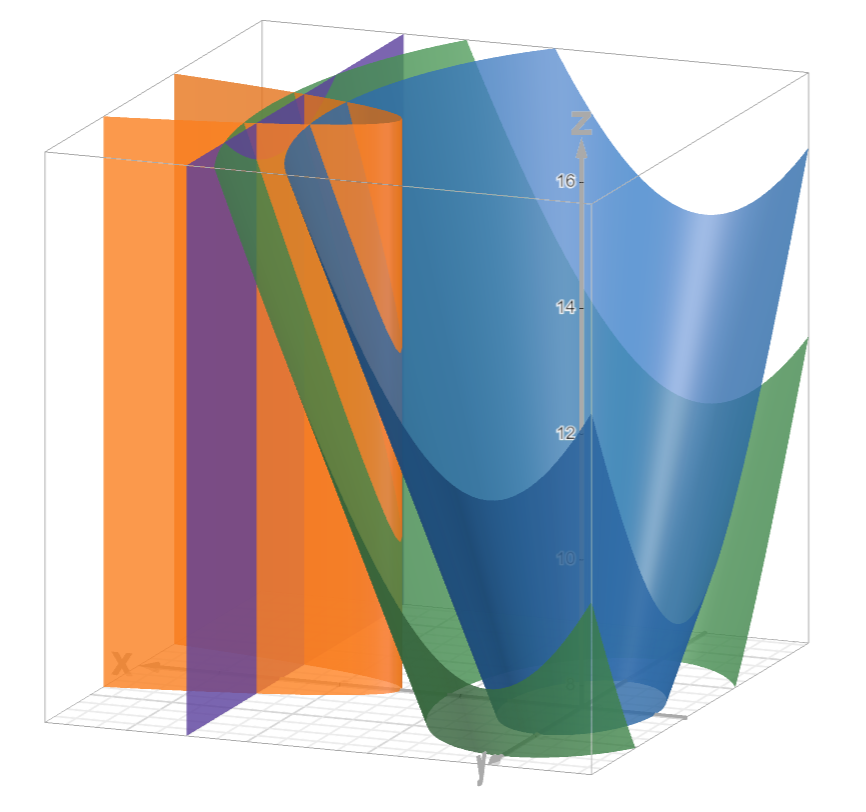
\includegraphics[width=0.4\linewidth]{Task3/Figure_outer_shapes.png}
    \caption{Задание 3. Ограничивающие поверхности \underline{\href{https://www.desmos.com/3D/kl5guofsih}{(Desmos)}}. }
\end{figure}
\newpage

\begin{figure}[h!t]
    \centering
    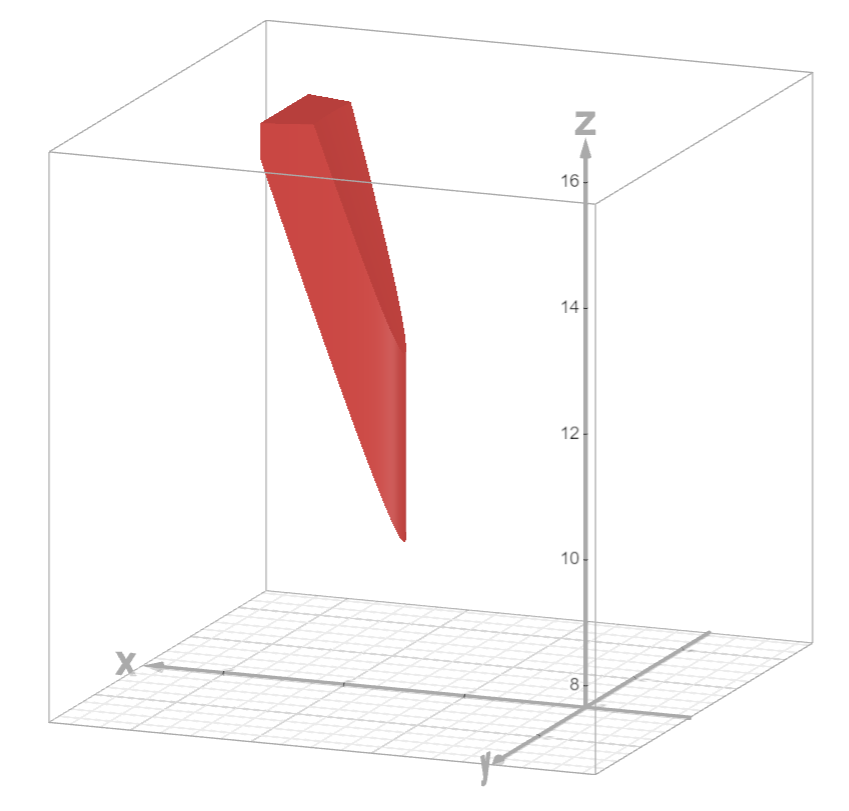
\includegraphics[width=0.6\linewidth]{Task3/Figure_volume_shape.png}
    \caption{Задание 3. Тело, которое задано поверхностями \underline{\href{https://www.desmos.com/3D/kl5guofsih}{(Desmos)}}. }
\end{figure}

\begin{figure}[h!t]
    \centering
    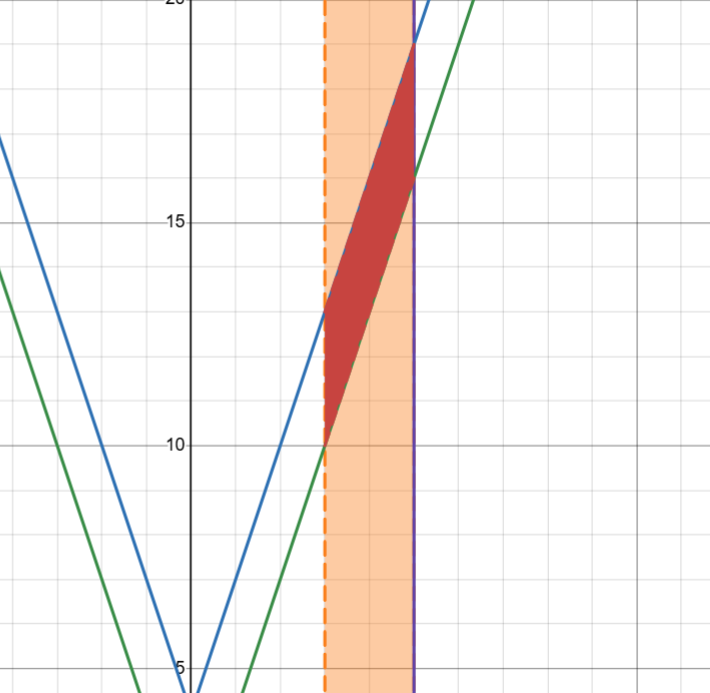
\includegraphics[width=0.6\linewidth]{Task3/Figure_XZ_intersection.png}
    \caption{Задание 3. Сечение по плоскости $XZ$ при $y=0$ \underline{\href{https://www.desmos.com/Calculator/q5wb8deh0a}{(Desmos)}}. }
\end{figure}

\newpage
\section{Задание 4.}

Сделать удобную замену переменных и найти площадь фигуры, выполнить
рисунок области.

$$    y = \frac{x^3}{a^2}, \quad y = \frac{x^3}{b^2}, \quad y = \frac{x^2}{c}, \quad y = \frac{x^2}{d}, \quad 0 < a < b, \quad 0 < c < d.$$

В идеале, нам нужно свести эту фигуру к прямоугольнику. Попробуем оставить параметры на одной части, переменные в другой.

$$ a^2 = \frac{x^3}{y}, \quad b^2 = \frac{x^3}{y}, \quad c = \frac{x^2}{y}, \quad d = \frac{x^2}{y}$$

Заметим, что для $a^2$ и $b^2$ уравнение повторяется, как и для $c$ и $d$.

$$ u = \dfrac{x^3}{y}\quad\quad v = \dfrac{x^2}{y} $$

Тогда эта область превращается в прямоугольник в $uv$ - плоскости, стороны которого ограничиваются сторонами $u=a^2$, $u=b^2$ и $v=c$ и $v=d$.

Можно посчитать площадь через следующий интеграл.

$$S = \int_{a^2}^{b^2} \int_{c}^{d} 1\cdot \left| \text{det}J\right| \,dv\,du$$

Где $\left|J\right|$ - это якобиан. Чтобы найти его, нужно выразить $x$ и $y$ через новые переменные. Сначала $x$.

$$
\begin{cases}
    u = \dfrac{x^3}{y}\,\vspace{1em}\\ 
    v = \dfrac{x^2}{y} 
\end{cases} \Rightarrow \quad
\begin{cases}
    y = \dfrac{x^3}{u}\,\vspace{1em}\\ 
    y = \dfrac{x^2}{v} 
\end{cases} \Rightarrow \quad
\dfrac{x^3}{u} = \dfrac{x^2}{v} \Rightarrow \quad
\dfrac{x^3}{x^2} = \dfrac{u}{v} \Rightarrow \quad
x = \dfrac{u}{v}
$$
Теперь $y$.
$$
\begin{cases}
    y = \dfrac{x^3}{u}\,\vspace{1em}\\ 
    x = \dfrac{u}{v}
\end{cases} \Rightarrow \quad 
y = \dfrac{u^3}{v^3} \cdot \dfrac{1}{u} = \dfrac{u^2}{v^3}
$$

Теперь посчитаем определитель якобиана.

$$\text{det}J = \text{det}\begin{pmatrix}
    \dfrac{\partial x}{\partial u} & \dfrac{\partial x}{\partial v} \vspace{1em}\\
    \dfrac{\partial y}{\partial u} & \dfrac{\partial y}{\partial v} 
\end{pmatrix}$$

$$\dfrac{\partial x}{\partial u} = \dfrac{\partial}{\partial u}\left(\dfrac{u}{v}\right) = \dfrac{1}{v} \quad\quad \dfrac{\partial x}{\partial v} = \dfrac{\partial}{\partial v}\left(\dfrac{u}{v}\right) = -\dfrac{u}{v^2}$$

$$\dfrac{\partial y}{\partial u} = \dfrac{\partial}{\partial u}\left( \dfrac{u^2}{v^3}\right) = \dfrac{2u}{v^3} \quad\quad \dfrac{\partial x}{\partial v} = \dfrac{\partial}{\partial v}\left(\dfrac{u^2}{v^3}\right) = -\dfrac{3u^2}{v^4}$$

Теперь подставим полученные значения в якобиан.

$$\text{det}\begin{pmatrix}
    \dfrac{\partial x}{\partial u} & \dfrac{\partial x}{\partial v} \vspace{1em}\\
    \dfrac{\partial y}{\partial u} & \dfrac{\partial y}{\partial v} 
\end{pmatrix} = \text{det}\begin{pmatrix}
    \dfrac{1}{v} & -\dfrac{u}{v^2} \vspace{1em}\\
    \dfrac{2u}{v^3} & -\dfrac{3u^2}{v^4}
\end{pmatrix} = \left( \frac{1}{v} \right) \left( -\frac{3u^2}{v^4} \right) - \left( -\frac{u}{v^2} \right) \left( \frac{2u}{v^3} \right) = \dfrac{u^2}{v^5}$$

Теперь вернемся к интегралу.

$$S = \int_{a^2}^{b^2} \int_{c}^{d} 1\cdot \left| \text{det}J\right| \,dv\,du = \int_{a^2}^{b^2} \int_{c}^{d} 1\cdot \left| - \dfrac{u^2}{v^5}\right| \,dv\,du = \int_{a^2}^{b^2} \int_{c}^{d} \dfrac{u^2}{v^5} \,dv\,du = $$

$$\int_{a^2}^{b^2} u^2 \,du\int_{c}^{d} \dfrac{1}{v^5} \,dv = \int_{a^2}^{b^2} u^2 \cdot \dfrac{1}{4v^4}\bigg|_{c}^d \,du = \int_{a^2}^{b^2} u^2 \dfrac{d^4 - c^4}{4c^4d^4} \,du = $$

$$= \dfrac{d^4 - c^4}{4c^4d^4} \int_{a^2}^{b^2} u^2 \,du = \dfrac{d^4 - c^4}{4c^4d^4} \cdot \dfrac{u^3}{3} \bigg|_{a^2}^{b^2} = \dfrac{d^4 - c^4}{4c^4d^4} \cdot \dfrac{b^6 - a^6}{3a^6b^6} =\boxed{\dfrac{(d^4 - c^4)(b^6 - a^6)}{12c^4d^4a^6b^6}}$$


\begin{figure}[h!t]
    \centering
    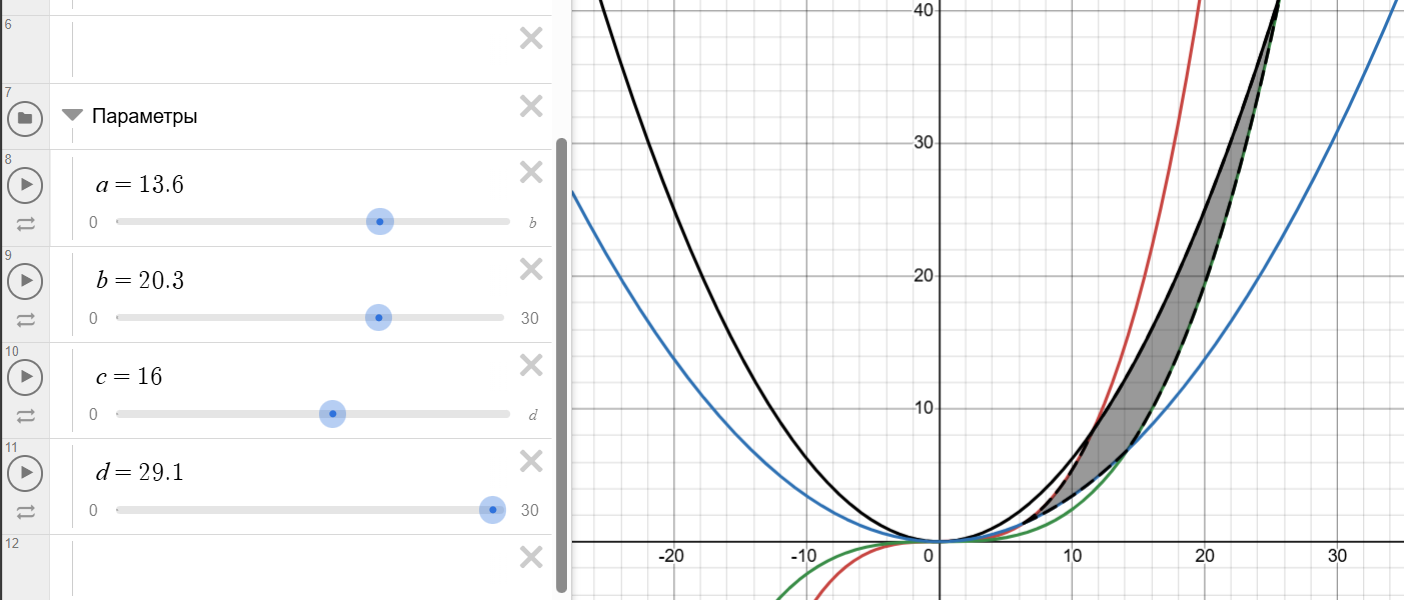
\includegraphics[width=1\linewidth]{Task4/graph.png}
    \caption{Задание 4. Изображение фигуры. \underline{\href{https://www.desmos.com/Calculator/5uewytafsp}{(Desmos)}}. }
\end{figure}
\newpage
\section{Задание 5.}

Найти объем тела, ограниченного поверхностями. Рисунок желателен. Па-
раметры считать положительными.
$$\left(x^{2}+y^{2}+z^{2}\right)^{3}=a^{6}\sin^{2}\left(\frac{\pi z}{\sqrt{x^{2}+y^{2}+z^{2}}}\right)$$
Тут напрашиваются сферические координаты. Сделаем переход.
$$
\begin{cases}
    x=r\sin{\theta}\cos{\phi}\\
    y=r\sin{\theta}\sin{\phi}\\
    z=r\cos{\theta}
\end{cases} \Rightarrow \quad \left(r^2\right)^{3}=a^{6}\sin^{2}\left(\frac{\pi r\cos{\theta}}{\sqrt{r^2}}\right) \Rightarrow \quad r^6 = a^6\sin^2\left(\pi\cos{\theta}\right) \quad \big/ \sqrt[6]{\text{     }}$$
$$r = a\sqrt[3]{\sin\left(\pi\cos{\theta}\right)}$$
Теперь мы знаем, что $r\in\left(0, a\sqrt[3]{\sin\left(\pi\cos{\theta}\right)}\right)$. Значит, мы можем записать интеграл.
$$\int_0^{2pi}\int_0^{\pi}\int_0^{a\sqrt[3]{\sin\left(\pi\cos{\theta}\right)}} \,dV = \int_0^{2pi}\int_0^{\pi}\int_0^{a\sqrt[3]{\sin\left(\pi\cos{\theta}\right)}} r^2\sin{\theta}\,dr\,d\theta \, d\phi =$$ 
$$=\int_0^{2pi}\, d\phi \int_0^{\pi} \sin{\theta}\,d\theta \int_0^{a\sqrt[3]{\sin\left(\pi\cos{\theta}\right)}} r^2\,dr = \int_0^{2pi}\, d\phi \int_0^{\pi}\dfrac{a^3}{3} \sin{\theta}\sin\left(\pi\cos{\theta}\right)\,d\theta = $$
\begin{center}    
    Сделаем замену переменной, пусть $u = \pi\cos{\theta}$, тогда $du = -\pi\sin{\theta}\,d\theta \Rightarrow -\dfrac{1}{\pi}\,du = \sin{\theta}\,d\theta$ 
    Насчет границ интегрирования: $\pi\cos{0} = \pi, \pi\cos{\pi} = -\pi$
\end{center}
$$\int_0^{2pi}\, d\phi \int_{\pi}^{-\pi}-\dfrac{a^3}{3\pi} \sin{u},du = \int_0^{2pi}\, d\phi \int_{-\pi}^{\pi}\dfrac{a^3}{3\pi} \sin{u},du \Rightarrow$$
\begin{center}    
    Синус нечетная функция, поэтому мы получим ноль. Но объем фигуры не может быть нулем, она просто симметрична относительно плоскости $XY$. Тогда поменяем границы интегрирования и удвоим интеграл.
\end{center}
$$\Rightarrow \int_0^{2pi}\, d\phi \int_{0}^{\pi}\dfrac{2a^3}{3\pi} \sin{u}\,du  = \dfrac{2a^3}{3\pi}\int_0^{2pi} \left[-\cos{u}\right]_0^{\pi}\, d\phi = \dfrac{2a^3}{3\pi}\int_0^{2pi} 2\, d\phi = \dfrac{2a^3}{3\pi} \cdot 4\pi =\boxed{\dfrac{8a^3}{3}}$$

\begin{figure}[h!t]
    \centering
    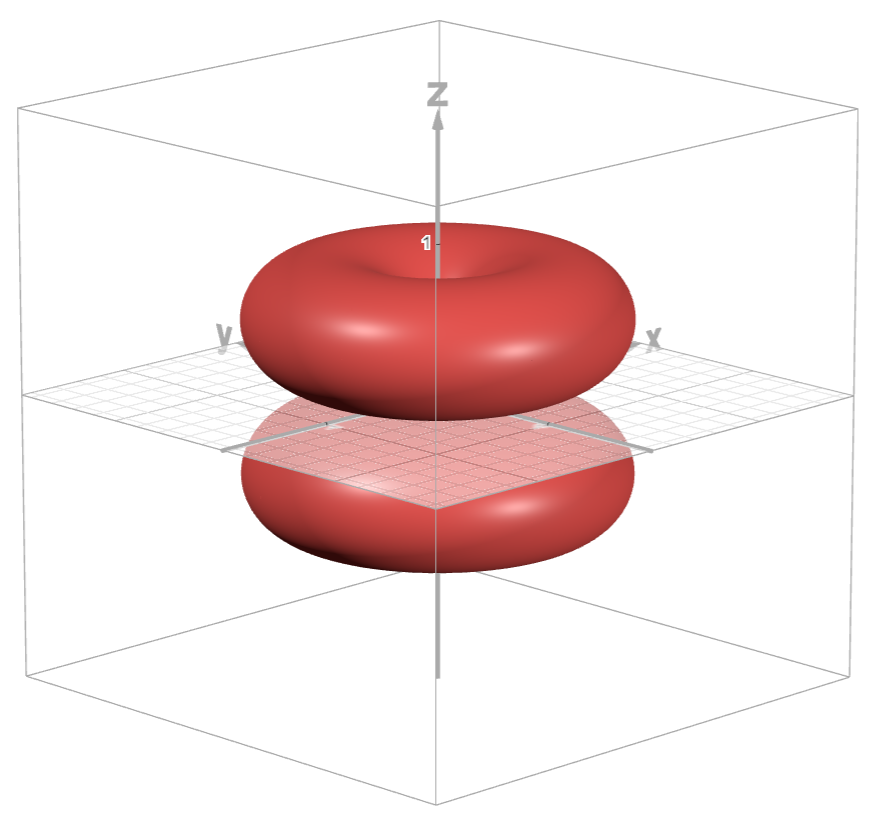
\includegraphics[width=0.5\linewidth]{Task5/Figure_shape.png}
    \caption{Задание 5. Изображение фигуры. \underline{\href{https://www.desmos.com/3D/hq9g3zataj}{(Desmos)}}. }
\end{figure}
\newpage
\section{Задание 6.}

Найти циркуляцию векторного поля $\vv{a}(x, y, z)$ вдоль замкнутого контура Г (ориентацию контура выбрать самостоятельно). Вычислить двумя способами:
с помощью криволинейного и поверхностного интегралов.

$$\vv{a} = y\vv{i} - x\vv{j} + z^2 \vv{k} \quad\text{Г}: z=3\left(x^2+y^2\right)+1, z = 4$$

Заметим, что контур Г можно упростить.

$$3\left(x^2+y^2\right)+1 = 4 \Rightarrow x^2+y^2 = 1^2$$

\subsection{Решение с помощью криволинейного интеграла.}

 Циркуляцию векторного поля $\vv{a}$ вдоль Г найдем по определению, как криволинейный интеграл второго рода.

 $$C(\vv{a}) =  \ointctrclockwise \limits_{\text{Г}} \vv{a} \cdot d\vv{r}$$

 Параметризуем наше уравнение.

 Путь, по которому мы проходим, назовем его $\gamma: \mathbb{R} \rightarrow \mathbb{R}^3$ параметризуем переменной $t$, $t\in(0, 2\pi)$.
 $$\gamma(t) = \left(\cos{t}, \sin{t}, 4\right)$$
 Касательная к этому пути будет $\gamma'(t)$.

 $$\gamma'(t) = \left(-\sin{t}, \cos{t}, 0\right)$$

Теперь, с помощью теоремы о вычислении КИ-2.

$$C(\vv{a})=\ointctrclockwise \limits_{\text{Г}} \vv{a} \cdot d\vv{r} = \int_0^{2\pi} \vv{a}(\gamma(t))\cdot\gamma'(t)\, dt$$

 Посчитаем подынтегральную функцию.
 $$\vv{a}(\gamma(t)) = \sin{t}\cdot\vv{i} - \cos{t}\cdot\vv{j} + 4^2$$
 $$\vv{a}(\gamma(t))\cdot\gamma'(t) = \left(\sin{t}, - \cos{t}, 16\right) \cdot \left(-\sin{t}, \cos{t}, 0\right) = -\sin^2{t}-\cos^2{t} + 16\cdot0 = -1$$
Тогда вернёмся к интегралу.

$$C(\vv{a}) = \int_0^{2\pi} \vv{a}(\gamma(t))\cdot\gamma'(t)\, dt = \int_0^{2\pi} -1 \, dt = \boxed{-2\pi}$$

\subsection{Решение с помощью поверхностного интеграла.}

Тут нам поможет т. Стокса, которая связывает циркуляцию с поверхностным интегралом (потоком). Пусть Г $= \partial\Sigma$

$$C_{\partial\Sigma}(\vv{a}) = \Pi_{\Sigma}(\vv{a}) \Rightarrow \ointctrclockwise \limits_{\partial\Sigma} \vv{a} \cdot d\vv{r} = \iint \limits_{\Sigma} \text{rot}\vv{a} \cdot \vv{N_0} d\vv{S}$$
\begin{center}
    Найдем ротор $\vv{a}$. По определению $\text{rot}\vv{a} = \nabla \times \vv{a}$
    
     $$\nabla \times \vv{a} = 
    \begin{vmatrix}
        \vv{i} & \vv{j} & \vv{k} \\
        \frac{\partial}{\partial x} & \frac{\partial}{\partial y} & \frac{\partial}{\partial z} \\
        y & -x & z^2 \\
    \end{vmatrix} =
    \left( \frac{\partial}{\partial y}\left(z^2\right) - \frac{\partial}{\partial z}\left(-x\right) \right) \vv{i} 
    - \left( \frac{\partial}{\partial x}\left(z^2\right) - \frac{\partial }{\partial z}\left(y\right) \right) \vv{j} 
    + \left( \frac{\partial }{\partial x}\left(-x\right) - \frac{\partial}{\partial y}\left(y\right) \right) \vv{k} =$$
    $$ =0 \vv{i} - 0 \vv{j} - 2\vv{k}$$
    Так как поверхность $\Sigma$ является просто диском, параллельным плоскости $XY$, то её вектор нормали в любой точке будет $N_0 = (0,0,1)$
    Осталось вспомнить, что $d\vv{S} = (dy\,dz, dx\,dz, dx\,dy)$
    
    Теперь посчитаем интеграл.
    
    $$\iint \limits_{\Sigma} \text{rot}\vv{a} \cdot \vv{N_0} d\vv{S} = \iint \limits_{\Sigma} \left((0,0,-2)\cdot(0,0,1) \right)\cdot(dy\,dz, dx\,dz, dx\,dy) = \iint \limits_{\Sigma} -2 dx \,dy = -2\iint \limits_{\Sigma} dx \,dy$$
    Причем этот двойной интеграл - это площадь круга с радиусом $1$, и он равен $\pi$.
    
    $$C_{\partial\Sigma}(\vv{a}) = -2\iint \limits_{\Sigma} dx \,dy = \boxed{-2\pi}$$
    
    Ответы сошлись, значит всё правильно :)
\end{center}

\newpage

\section{Задание 7.}

Найти поток векторного поля $\vv{a}(x, y, z)$ через замкнутую поверхность S (нормаль внешняя). Вычислить двумя способами: с помощью поверхностного и тройного интеграла.

$$\vv{a} = y\vv{i} + 5y\vv{j} + z\vv{k}, \quad S: x^2 + y^2 = 1, \quad z = x, \quad z = 0, \quad z \geq 0$$

\begin{figure}[h!t]
    \centering
    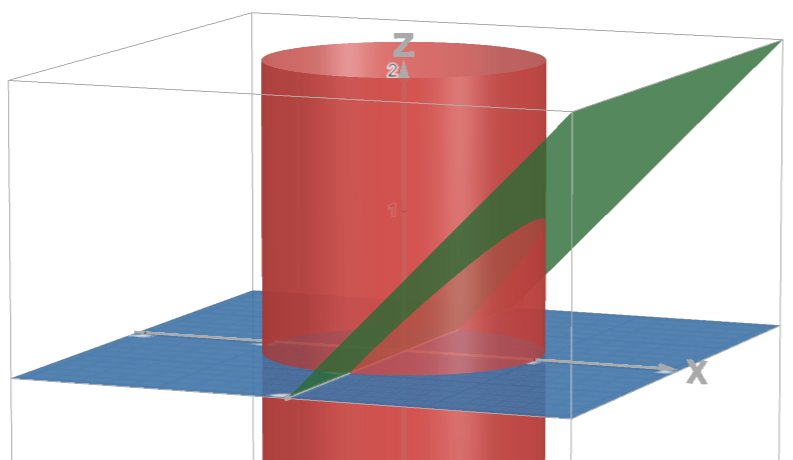
\includegraphics[width=0.5\linewidth]{Task7/Surfaces_closing_the_figure.png}
    \caption{Задание 7. Поверхности, задающие фигуру.\underline{\href{https://www.desmos.com/3d/pfnmmjbtkb}{(Desmos)}}.}
\end{figure}

\subsection{Решение с помощью тройного интеграла.}

Воспользуемся теоремой Остроградского-Гаусса.

$$\Pi_S(\vv{a}) = \iint \limits_S \vv{a} \cdot \vv{N_0} \, dS = \iiint \limits_V (\text{div}\vv{a})\,dV$$

Посчитаем дивергенцию векторного поля $\vv{a}$.
$$\text{div}\vv{a} = \nabla \cdot \vv{a} = \dfrac{\partial}{\partial x}\left(y\right) + \dfrac{\partial}{\partial y}\left(5y\right) + \dfrac{\partial}{\partial z}\left(z\right) = 0 + 5 + 1 = 6$$

Теперь подставим.

$$\iiint \limits_V (\text{div}\vv{a})\,dV = 6 \iiint \limits_V \,dV$$

Перейдем в цилиндрические координаты. Причем, для нашей фигуры нужно ограничить переменные следующим образом. 
$$
\begin{cases}
    x=r\cos{\phi}\\
    y=r\sin{\phi}\\
    z=z
\end{cases} ; \quad
\begin{cases}
    z\geq0\\
    z=x
\end{cases} \Rightarrow \quad
\begin{cases}
    z\geq0\\
    z = r\cos{\phi}
\end{cases} \Rightarrow \quad
\begin{cases}
    \cos{\phi} \geq 0 \\
    \phi \in [-\pi/2, \pi/2]
\end{cases} \Rightarrow \quad
\begin{cases}
    r \in [0,1]\\
    \phi \in [-\pi/2, \pi/2]\\
    z\in[0, r\cos{\phi}]
\end{cases}$$

Теперь мы можем сделать замену, учитывая $\left| J\right| = r$ 

$$6 \iiint \limits_V \,dV = 6 \int_0^1\,dr \int_{-\pi/2}^{\pi/2} \,d\phi \int_0^{r\cos{\phi}} r\, dz = 6 \int_0^1\,dr \int_{-\pi/2}^{\pi/2} r^2\cos{\phi}\,d\phi = 6 \int_0^1 r^2 \left[-\sin{\phi}\right]_{-\pi/2}^{\pi/2} \,dr =$$ 
$$= 6 \int_0^1 r^2 \cdot 2 \,dr = 12 \cdot \dfrac{1}{3} = \boxed{4}.$$


\subsection{Решение с помощью поверхностного интеграла.}

$$\Pi_S(\vv{a}) = \iint \limits_S \vv{a} \cdot \vv{N_0} d\vv{S}$$

По свойству аддитивности интеграла, разобьем его на три: нижняя крышка, кусок цилиндра и верхняя крышка. 

$$\iint \limits_S = \iint \limits_{\text{нижняя крышка}} + \iint \limits_{\text{верхняя крышка}} + \iint \limits_{\text{кусок цилиндра}}$$
\begin{center}

Теперь найдем векторы нормали для каждого интеграла.
\begin{figure}[h!t]
    \centering
    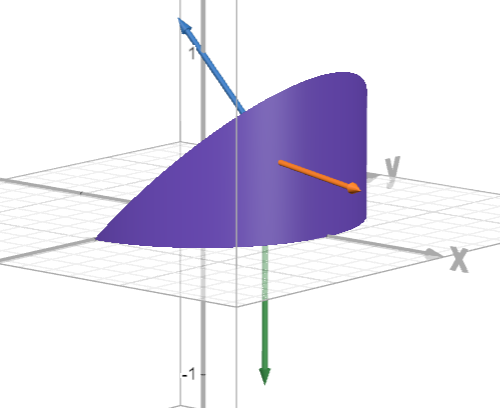
\includegraphics[width=0.5\linewidth]{Task7/Normal_vectors_of_the_figure.png}
    \caption{Задание 7. Векторы нормали фигуры. \underline{\href{https://www.desmos.com/3d/aebkcx5iql}{(Desmos)}}.}
\end{figure}

    Для нижней крышки (зеленая стрелка) $\vv{N_0} = (0,0,-1)$\\
    Для верхней крышки (синяя стрелка) $\vv{N_0} = (-\sqrt{2}/2, 0,\sqrt{2}/2)$\\
    Для куска цилиндра (оранжевая стрелка) $\vv{N_0}(\phi) = (\cos{\phi}, \sin{\phi}, 0)$

Теперь можно рассмотреть каждый интеграл по отдельности.

$$\iint \limits_{\text{нижняя крышка}} \vv{a} \cdot \vv{N_0} d\vv{S} = 
\iint \limits_{\text{нижняя крышка}} (y,5y,z) \cdot (0,0,-1) d\vv{S} = 
\iint \limits_{\text{нижняя крышка}} -z\, d\vv{S} = 0$$

Так как нижняя крышка задается уравнением $z=0$, то этот интеграл будет равен нулю.

$$\iint \limits_{\text{верхняя крышка}} \vv{a} \cdot \vv{N_0} d\vv{S} = \iint \limits_{\text{верхняя крышка}} (y,5y,z) \cdot (-\sqrt{2}/2, 0,\sqrt{2}/2) d\vv{S} = \dfrac{\sqrt{2}}{2} \iint \limits_{\text{верхняя крышка}} (-y + z) d\vv{S}$$

Мы можем выразить $z$ через $x$, т.к. эта поверхность задается уравнением $z=x$. Теперь $z(x,y) = x$.

$$d\vv{S} = \sqrt{1 + \left(\frac{\partial z}{\partial x}\right)^2 + \left(\frac{\partial z}{\partial y}\right)^2} \,dx\,dy = \sqrt{1 + \left(\frac{\partial x}{\partial x}\right)^2 + \left(\frac{\partial x}{\partial y}\right)^2} \,dx\,dy = \sqrt{2}\,dx\,dy$$

$$\dfrac{\sqrt{2}}{2} \iint \limits_{\text{верхняя крышка}} (-y + z) d\vv{S} = \sqrt{2} \cdot \dfrac{\sqrt{2}}{2} \iint \limits_{x^2 + y^2\leq1 \{x\geq0\}} (-y + x) \,dx\,dy$$
Перейдем в полярные координаты.
$$\iint \limits_{x^2 + y^2\leq1 \{x\geq0\}} (-y + x) \,dx\,dy = \int_{-\pi/2}^{\pi/2} d\phi \int_0^1 (-r\sin{\phi} + r\cos{\phi}) \cdot r \, dr = \dfrac{1}{3}\int_{-\pi/2}^{\pi/2} \cos{\phi} - \sin{\phi}\,d\phi = $$

$$= \dfrac{1}{3} \left[\sin{\phi}+\cos{\phi}\right]_{-\pi/2}^{\pi/2} = \dfrac{1}{3} \left[1+0-(-1+0)\right] = \dfrac{2}{3}$$

Теперь последний интеграл.
Сразу перейдем в цилиндрические координаты, чтобы можно было пользоваться вектором нормали. Тут $r=const=1$, тогда $|J| = 1$.

$$
\begin{cases}
    x=\cos{\phi}\\
    y=\sin{\phi}\\
    z=z
\end{cases}
$$
Так как эта поверхность ограничена сверху плоскостью $z=x$, можно выразить $z$ через $x$.

$$
\begin{cases}
    x=\cos{\phi}\\
    z=x
\end{cases}\Rightarrow \quad z\in[0, \cos{\phi}]
$$
$$\iint \limits_{\text{кусок цилиндра}} \vv{a} \cdot \vv{N_0} d\vv{S} = 
\int_{-\pi/2}^{\pi/2}\, d\phi \int_{0}^{\cos{\phi}} \left((\sin{\phi}, 5\sin{\phi}, z) \cdot (\cos{\phi}, \sin{\phi}, 0)\right)\,dz = $$
$$=\int_{-\pi/2}^{\pi/2}\, \left(\sin{\phi}\cos{\phi} +  5\sin^2{\phi}\right)\cos{\phi}\, d\phi = \int_{-\pi/2}^{\pi/2}\, \sin{\phi}\cos^2{\phi} + 5\sin^2{\phi}\cos{\phi}\, d\phi = $$ 
$$= \int_{-\pi/2}^{\pi/2} \sin{\phi}\cos^2{\phi}\, d\phi + \int_{-\pi/2}^{\pi/2} 5\sin^2{\phi}\cos{\phi}\, d\phi$$

Рассмотрим левый интеграл и сразу сделаем замену переменной пусть $u=\cos{\phi}$, $du = -\sin{\phi}\,d\phi$
$$\int_{-\pi/2}^{\pi/2} \sin{\phi}\cos^2{\phi}\, d\phi = -\int_{0}^{0} u^2\, du = 0$$

Рассмотрим правый интеграл и сразу сделаем замену переменной пусть $u=\sin{\phi}$, $du = \cos{\phi}\,d\phi$

$$\int_{-\pi/2}^{\pi/2} 5\sin^2{\phi}\cos{\phi}\, d\phi = \int_{-1}^{1} 5u^2 \, du = 5 \cdot \left[\dfrac{u^3}{3}\right]_{-1}^1 = 5 \cdot \left[\dfrac{1}{3} - \left(-\dfrac{1}{3}\right)\right] = \dfrac{10}{3}$$

Теперь сложим полученные значения трех интегралов.

$$0 + \dfrac{2}{3} + \dfrac{10}{3} = \dfrac{12}{3} = \boxed{4}$$

Ответы сошлись, значит всё правильно :)

\end{center}

\newpage
\section{Задание 8.}

Найти поток векторного поля $\vv{a}(x, y, z)$ через замкнутую поверхность S (нормаль внешняя). Вычислить двумя способами: с помощью поверхностного и тройного интеграла.

 $$\vv{a} =3xz\vv{i} - 2x\vv{j}+y\vv{k},\quad S: x+y+z = 2, x=1, x=0, y =0, z =0$$

\subsection{Решение с помощью тройного интеграла.}

Воспользуемся теоремой Остроградского-Гаусса.

$$\Pi_S(\vv{a}) = \iint \limits_S \vv{a} \cdot \vv{N_0} \, dS = \iiint \limits_V (\text{div}\vv{a})\,dV$$

Посчитаем дивергенцию векторного поля $\vv{a}$.
$$\text{div}\vv{a} = \nabla \cdot \vv{a} = \dfrac{\partial}{\partial x}\left(3xz\right) + \dfrac{\partial}{\partial y}\left(- 2x\right) + \dfrac{\partial}{\partial z}\left(y\right) = 3z + 0 + 0 = 3z$$
\begin{center}
    
Теперь подставим.

$$\iiint \limits_V (\text{div}\vv{a})\,dV = \iiint \limits_V 3z \,dV$$

Теперь определимся с границами интегрирования. $x\in[0,1]$, $y\in[0,\leq 2-x]$, $z\in[0,2-x-y]$

$$\iiint \limits_V 3z \,dV = \int_0^1 \, dx \int_{0}^{2-x}\,dy \int_{0}^{2-x-y} 3z\, dz$$

Интегрируем по $z$.
$$ \int_{0}^{2-x-y} 3z \, dz = 3\left[ \frac{z^2}{2} \right]_{0}^{2-x-y} = \frac{3(2-x-y)^2}{2} $$
Интегрируем по $y$.
$$ \int_{0}^{2-x} \frac{3(2-x-y)^2}{2} \, dy = \frac{3}{2} \int_{0}^{2-x} (4 - 4x - 4y + x^2 + 2xy + y^2) \, dy = \frac{3}{2} \left[ 4y - 4xy - 2y^2 + x^2y + xy^2 + \frac{y^3}{3} \right]_{0}^{2-x} =$$
$$ =\frac{1}{2} \left[ 12y - 12xy - 6y^2 + 3x^2y + 3xy^2 + y^3\right]_{0}^{2-x} =$$ 
$$=\frac{1}{2} \left[ 12(2-x) - 12x(2-x) - 6(2-x)^2 + 3x^2(2-x) + 3x(2-x)^2 + (2-x)^3\right] = ... =$$ 
$$=\frac{1}{2}\left[-x^3 + 6x^2 - 12x + 8\right]$$
Интегрируем по $x$.
$$\frac{1}{2}\int_0^1 -x^3 + 6x^2 - 12x + 8\, dx = \frac{1}{2}\left[ \frac{x^4}{4} + 2x^3 - 6x^2 + 8x \right]_0^1 = \frac{1}{2}\left( -\frac{1^4}{4} + 2 \cdot 1^3 - 6 \cdot 1^2 + 8 \cdot 1 \right) =$$
$$=\frac{1}{2}\left(-\frac{1}{4} + 2 - 6 + 8\right) = \frac{1}{2}\cdot\frac{-1 + 8 - 24 + 32}{4} = \boxed{\frac{15}{8}}$$
\end{center}

\newpage
\subsection{Решение с помощью поверхностного интеграла.}

$$\Pi_S(\vv{a}) = \iint \limits_S \vv{a} \cdot \vv{N_0} d\vv{S}$$


\begin{figure}[h!t]
    \centering
    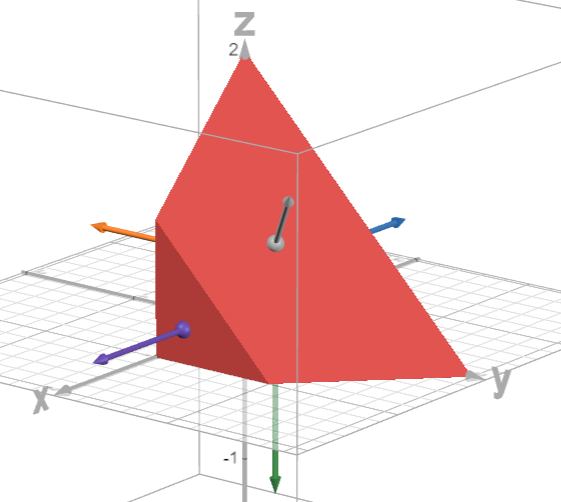
\includegraphics[width=0.75\linewidth]{Task8/Normal_vectors.png}
    \caption{Задание 8. Форма фигуры, с её векторами нормали.\underline{\href{https://www.desmos.com/3D/p0j1s5t0mn}{(Desmos)}}.}
\end{figure}
\begin{center}


Разделим интеграл на 5 поверхностей.

$$\iint \limits_S = \iint \limits_{\text{верхняя}} + \iint \limits_{\text{передняя}} + \iint \limits_{\text{левая}} + \iint \limits_{\text{задняя}} + \iint \limits_{\text{нижняя}}$$
Теперь перейдем к самой увлекательной части.

$$\iint \limits_{\text{верхняя}} \vv{a} \cdot \vv{N_0} d\vv{S} = \dfrac{1}{\sqrt{3}}\iint \limits_{\text{верхняя}} (3xz, - 2x, + y) \cdot (1,1,1))\, d\vv{S} = \dfrac{1}{\sqrt{3}}\iint \limits_{\text{верхняя}} 3xz - 2x + y\, d\vv{S}$$$$\begin{cases}
    z(x,y)=2-x-y\\
    d\vv{S} = \sqrt{1 + \left(\frac{\partial z}{\partial x}\right)^2 + \left(\frac{\partial z}{\partial y}\right)^2}\,dx\,dy
\end{cases} \Rightarrow \quad d\vv{S} = \sqrt{1 + (-1)^2 + (-1)^2}\,dx\,dy = \sqrt{3}\,dx\,dy$$
$$= \sqrt{3}\cdot\dfrac{1}{\sqrt{3}} \int_0^1\,dx \int_0^{2-x} 3x(2-x-y) - 2x + y\,dy = \int_0^1\,dx\int_{0}^{2-x} (4x - 3x^2 - 3xy + y) \, dy = $$
$$=\int_0^1\left[ (4x - 3x^2)y - \frac{3xy^2}{2} + \frac{y^2}{2} \right]_{0}^{2-x}\,dx =\int_0^1 (4x - 3x^2)(2 - x) - \frac{3x(2 - x)^2}{2} + \frac{(2 - x)^2}{2}\,dx =  $$
$$ \int_{0}^{1} \left( 2 + \frac{3x^3}{2} - \frac{7x^2}{2} \right) \, dx = \left[ 2x + \frac{3x^4}{8} - \frac{7x^3}{6} \right]_{0}^{1} = \left( 2 + \frac{3}{8} - \frac{7}{6} \right) = \left( 2 + \frac{9}{24} - \frac{28}{24} \right) =$$ 
$$= \left( 2 - \frac{19}{24} \right) = \left( \frac{48}{24} - \frac{19}{24} \right) = \frac{29}{24} $$

$$\iint \limits_{\text{передняя}} \vv{a} \cdot \vv{N_0}\, d\vv{S} = \iint \limits_{\text{передняя}} (3xz, - 2x, + y) \cdot (1,0,0))\, d\vv{S} =\iint \limits_{\text{передняя}} 3xz\, d\vv{S} = \int_0^1\,dy \int_0^{1-y} 3xz\,dz = $$
$$=\left\{\text{тут $x=const=1$}\right\} = 3\int_0^1\,dy \int_0^{1-y} z\,dz = \dfrac{3}{2}\int_0^1 (1-y)^2 \,dy = \dfrac{3}{2}\left[y - y^2 + \dfrac{y^3}{3}\right]_0^1 = \dfrac{3}{2}\left[1 - 1 + \dfrac{1}{3}\right] = \dfrac{1}{2}$$

$$\iint \limits_{\text{левая}} \vv{a} \cdot \vv{N_0}\, d\vv{S} = \iint \limits_{\text{левая}} (3xz, - 2x, + y) \cdot (0,-1,0))\, d\vv{S} = \iint \limits_{\text{левая}}2x\, d\vv{S} = \int_0^1\, dx \int_0^{2-x} 2x\,dz = $$ 
$$ = \int_0^1 2x(2-x) \, dx = 2\int_0^1 2x-x^2 \, dx = 2\left[x^2 - \dfrac{x^3}{3}\right]_0^1 = 2\left[1 - \dfrac{1}{3}\right] = \dfrac{4}{3}$$

$$\iint \limits_{\text{задняя}} \vv{a} \cdot \vv{N_0}\, d\vv{S} = \iint \limits_{\text{задняя}} (3xz, - 2x, + y) \cdot (-1,0,0))\, d\vv{S} = \iint \limits_{\text{задняя}} -3xz\, d\vv{S} = $$ 
$$ = \left\{\text{тут $x=0$ на всей поверхности}\right\} = 0$$ 

$$\iint \limits_{\text{нижняя}}\vv{a} \cdot \vv{N_0}\, d\vv{S} = \iint \limits_{\text{нижняя}} (3xz, - 2x, + y) \cdot (0,0,-1))\, d\vv{S} = \iint \limits_{\text{нижняя}} -y \,d\vv{S} = -\int_0^1\, dx \int_0^{2-x} y\,dy = $$
$$ = -\dfrac{1}{2}\int_0^1 (2-x)^2 \, dx = -\dfrac{1}{2}\int_0^1 4-4x+x^2 \, dx = -\dfrac{1}{2}\left[4x - 2x^2 + \dfrac{x^3}{3}\right]_0^1 = -\dfrac{1}{2}\left[4 - 2 + \dfrac{1}{3}\right] = -\dfrac{7}{6}$$

$$\iint \limits_S \vv{a} \cdot \vv{N_0} d\vv{S} = \frac{29}{24} + \frac{1}{2} + \dfrac{4}{3} + 0 - \dfrac{7}{6} = \boxed{\dfrac{15}{8}}$$

Ответы сошлись, мы победили :)

\end{center}

\newpage
\section{Задание 9.}

Проверить, является ли данное поле потенциальным и соленоидальным. Для потенциального поля найти его потенциал с помощью криволинейного интеграла. Провести проверку потенциала.

$$\vv{a} = (2x \sin y - 2) \vv{i} + (x^2 \cos y - z^2) \vv{j} - 2yz \vv{k}.$$

Воспользуемся критерием потенциальности поля и проверим, что его ротор равен нулю.
$$\nabla \times \vv{a} = 
\begin{vmatrix}
\vv{i} & \vv{j} & \vv{k} \\
\dfrac{\partial}{\partial x} & \dfrac{\partial}{\partial y} & \dfrac{\partial}{\partial z} \\
2x \sin y - 2 & x^2 \cos y - z^2 & -2yz \\
\end{vmatrix}$$

$$\nabla \times \vv{a} = \left( \frac{\partial}{\partial y} (-2yz) - \frac{\partial}{\partial z} (x^2 \cos y - z^2) \right) \vv{i} - \left( \frac{\partial}{\partial x} (-2yz) - \frac{\partial}{\partial z} (2x \sin y - 2) \right) \vv{j} +$$
$$ +\left( \frac{\partial}{\partial x} (x^2 \cos y - z^2) - \frac{\partial}{\partial y}(2x \sin y - 2)\right) \vv{k} = (-2z - (-2z)) \vv{i} - (0 - 0) \vv{j} + (2x \cos y - 2x \cos y) \vv{k} =$$
$$=0\vv{i} + 0\vv{j} + 0\vv{k} = 0 \Rightarrow \text{Поле потенциально.}$$

Воспользуемся критерием соленоидальности поля и проверим, что его дивергенция равна нулю.

$$\nabla \cdot \vv{a} = \frac{\partial}{\partial x}(2x \sin y - 2) + \frac{\partial}{\partial y}(x^2 \cos y - z^2) + \frac{\partial}{\partial z}(-2yz)= $$
$$= 2 \sin y + (-x^2 \sin y) + (-2y) = 2 \sin y - x^2 \sin y - 2y \neq \Rightarrow \text{Поле \textbf{не} солеидально.}0$$

Теперь найден потенциал поля. Для этого нужно найти интеграл по этому полю от $(x_0, y_0, z_0)$ до $(x,y,z)$. Так как поле потенциально, криволинейный интеграл не зависит от пути, поэтому возьмем точку $(0,0,0)$. Пусть $\phi$ - потенциал поля, т.е. $\vv{a} = \text{grad}\phi$
$$\frac{\partial \phi}{\partial x} = 2x \sin y - 2, \quad \frac{\partial \phi}{\partial y} = x^2 \cos y - z^2, \quad \frac{\partial \phi}{\partial z} = -2yz$$

Будем действовать по чуть-чуть, по одной переменной. Так как нам нужно воспользоваться криволинейным интегралом, то запишем одну идею.

$$\phi(x,y,z) = \int 2x \sin y - 2\, dx = 2x^2 \sin y - 2x +  f(y,z)$$
Тут $f$ - это какая-то функция двух переменных $y$ и $z$ (чтобы $\frac{\partial f}{\partial x} = 0$). Потом мы придумаем $g(z)$, чтобы $\frac{\partial g}{\partial y} = 0$. Чтобы сделать это в виде криволинейного интеграла, запишем так.

$$\phi(x,y,z) = \int_\gamma \text{, где $\gamma$ - путь от $(0,0,0)$ до $(x,y,z)$}$$

$$\int_\gamma = \int_0^x \vv{a_x}(t,0,0)\,dt + \int_0^y \vv{a_x}(x,t,0)\,dt + \int_0^z \vv{a_x}(x,y,t)\,dt$$

$$\int_0^x \vv{a_x}(t,0,0)\,dt = \int_0^x 2t \sin 0 - 2\,dt = \int_0^x (- 2)\,dt = -2x$$

$$\int_0^y \vv{a_y}(x,t,0)\,dt = \int_0^y x^2 \cos{t} - 0^2 \,dt =x^2 \sin{y} $$

$$\int_0^z \vv{a_z}(x,y,t)\,dt =\int_0^z -2yt\,dt = -yz^2$$

$$\text{Тогда } \phi(x,y,z) = -2x + x^2 \sin{y} - yz^2$$
\begin{center}
    Сделаем проверку $\vv{a} = \text{grad}\phi$.
\end{center}

$$\text{grad}\phi = \left(\dfrac{\partial \phi}{\partial x},\dfrac{\partial \phi}{\partial y}, \dfrac{\partial \phi}{\partial z} \right)$$

$$\dfrac{\partial \phi}{\partial x} = \dfrac{\partial}{\partial x}\left(-2x + x^2 \sin{y} - yz^2\right) = -2 + 2x\sin{y}$$

$$\dfrac{\partial \phi}{\partial y} = \dfrac{\partial}{\partial y}\left(-2x + x^2 \sin{y} - yz^2\right) = x^2\cos{y} - z^2$$

$$\dfrac{\partial \phi}{\partial z} = \dfrac{\partial}{\partial z}\left(-2x + x^2 \sin{y} - yz^2\right) = -2yz$$
\begin{center}
    Действительно, $\text{grad}\phi = \vv{a}$, значит у нас еще одна победа.
\end{center}
    
\newpage
\section{Задание 10.}

Вычислить данный криволинейный интеграл аналитически двумя способами, а также численно двумя способами.

$$\varointclockwise_L xy^2 \,dx - x^2y \,dy, \quad L \text{ - граница полукруга } D: x^2 + y^2 \leq 16, x + y \leq 0$$

\subsection{Аналитический способ.}
\subsubsection{С помощью формулы Грина.}
\begin{center}
    
Теорема грина гласит, что для функций $P,Q \in C^1(\text{cl}D)$.

$$\ointctrclockwise_{L} P \, dx + Q \, dy = \iint_{D} \left( \dfrac{\partial Q}{\partial x} - \dfrac{\partial P}{\partial y} \right)\,dx\,dy$$

В нашем случае, $P=xy^2, Q=-x^2y. \quad P,Q \in C^1(\mathbb{R})$

$$\dfrac{\partial Q}{\partial x} = \dfrac{\partial}{\partial x}\left(-x^2y\right) = -2xy \quad\quad \dfrac{\partial P}{\partial y} = \dfrac{\partial}{\partial y}\left(xy^2\right) = 2xy $$

Теперь нужно поменять знак двойного интеграла, потому что мы идем в отрицательном направлении.

$$ \varointclockwise_L xy^2 \,dx - x^2y \,dy = - \iint_D (-2xy - 2xy)\,dx\,dy = \iint_D 4xy \,dx\,dy = 4\iint_D xy \,dx\,dy$$

Перейдем в полярные координаты. 

$$
\begin{cases}
    x^2+y^2 \leq 16 = 4^2\\
    x+y\leq0
\end{cases} \Rightarrow\quad 
\begin{cases}
    x = r\cos{\phi}\\
    y = r\sin{\phi}\\
    r\in[0, 4]\\
    r\cos{\phi}+r\sin{\phi}\leq0
\end{cases} \Rightarrow\quad 
\cos{\phi}+\sin{\phi}\leq0 \Rightarrow\quad \phi\in\left[\dfrac{3\pi}{4}, \dfrac{7\pi}{4} \right]
$$

$$4\iint_D xy \,dx\,dy = \int_0^4 dr \int_{3\pi/4}^{7\pi/4} r^2\cos{\phi}\sin{\phi} \,d\phi = \dfrac{1}{2}\int_0^4 r^2\,dr\int_{3\pi/4}^{7\pi/4} \sin{2\phi} \,d\phi = $$
$$=\dfrac{1}{4}\int_0^4 r^2\,dr\int_{3\pi/4}^{7\pi/4} \sin{2\phi} \,d2\phi = \dfrac{1}{4}\int_0^4 r^2 \left[ \cos{2\phi} \right]_{3\pi/4}^{7\pi/4}  \,dr  = \dfrac{1}{4}\int_0^4 r^2 \left[ 0-0 \right]\,dr = \boxed{0} $$
\end{center}

\subsubsection{С помощью т. О вычислении КИ-2.}

$$\varointclockwise_L xy^2 \,dx - x^2y \,dy$$
\begin{center}
    
Пусть $\vv{F} = (F_1, F_2) = (xy^2, - x^2y), \quad d\vv{r} = (dx,dy), \quad \gamma(t): \mathbb{R} \rightarrow \mathbb{R}^2$ - путь по $L$.

$$\varointclockwise_L xy^2 \,dx - x^2y \,dy = \varointclockwise_L \vv{F} \cdot d\vv{r} = \int_a^b \left(F(\gamma(t))\cdot\gamma'(t)\right)dt$$

\begin{figure}[h!t]
    \centering
    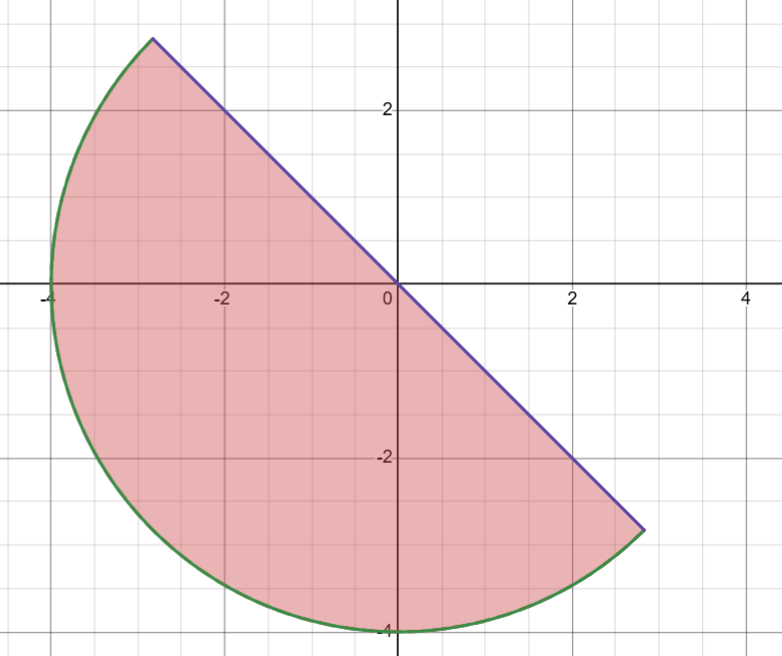
\includegraphics[width=0.75\linewidth]{Task10/Figure_D.png}
    \caption{Задание 10. Область D.}
    \label{task-10:figure-D}
\end{figure}

Разобьем кривую $L$ на две: $L_1$ и $L_2$ и присвоим им соответствующие пути $\gamma_1(t)$ и $\gamma_2(t)$. Пусть $\gamma_1$ проходит по прямой $y=-x$, на рисунке \ref{task-10:figure-D} он показан фиолетовым. Тогда $\gamma_2$ проходит по зеленой полуокружности, по часовой стрелке.
$$\gamma_1(t) = (t,-t), \quad t\in[-2\sqrt{2}, 2\sqrt{2}]$$
$$\gamma_2(t) = (4\sin{t}, 4\cos{t}), \quad t\in[3\pi/4, 7\pi/4]$$
$$\gamma_1'(t) = (1,-1), \quad \gamma_2'(t) = (4\cos{t}, -4\sin{t})$$


В $\gamma_2$ мы поменяли синус и косинус местами, чтобы он шел в правильном направлении, по часовой стрелке.

$$\varointclockwise_L \vv{F} \cdot d\vv{r} = \varointclockwise_{L_1} \vv{F} \cdot d\vv{r} + \varointclockwise_{L_2} \vv{F} \cdot d\vv{r} = \int_{-2\sqrt{2}}^{2\sqrt{2}} \left(F(\gamma_1(t))\cdot\gamma_1'(t)\right)dt + \int_{3\pi/4}^{7\pi/4} \left(F(\gamma_2(t))\cdot\gamma_2'(t)\right)dt = $$

$$= \int_{-2\sqrt{2}}^{2\sqrt{2}} \left((t(-t)^2, - t^2(-t)) \cdot (1,-1)) \right)\, dt +$$ 
$$+\int_{3\pi/4}^{7\pi/4} \left((4\sin{t})(4\cos{t})^2, - (4\sin{t})^2(4\cos{t}))\cdot(4\cos{t}, -4\sin{t})\right)\,dt = $$
$$= \int_{-2\sqrt{2}}^{2\sqrt{2}} t^3 - t^3\, dt + \int_{3\pi/4}^{7\pi/4} 256\sin{t}\cos^3{t} + 256\sin^3{t}\cos{t}\,dt =$$
$$= \int_{-2\sqrt{2}}^{2\sqrt{2}} 0\, dt + 256\int_{3\pi/4}^{7\pi/4} \sin{t}\cos{t}(\cos^2{t} + \sin^2{t})\,dt =256\int_{3\pi/4}^{7\pi/4} \sin{t}\cos{t}\,dt =$$
$$= 128\int_{3\pi/4}^{7\pi/4} \sin{2t}\,dt = 64\int_{3\pi/4}^{7\pi/4} \sin{2t}\,d2t = 64\left[ \cos{2\phi} \right]_{3\pi/4}^{7\pi/4} = 64[0-0]= \boxed{0}$$
\end{center}

\newpage
\subsection{Численный метод.}
\subsubsection{Результаты вычислений:}

\begin{table}[h!t]
    \centering
    \begin{tabular}{|c|c|c|c|}
    \hline
    $\delta$ & интегральная сумма & отклонение & время выполнения (c)\\
    \hline
    0.1 & -0.035333 & -0.035333 & 0.000272\\
    \hline
    0.01 & -0.00037 & -0.00037 & 0.002479\\
    \hline
    0.001 & -4e-06 & -4e-06 & 0.02521\\
    \hline
\end{tabular}

    \caption{Криволинейный интеграл.}
\end{table}

\begin{table}[h!t]
    \centering
    \begin{tabular}{|c|c|c|c|}
    \hline
    $\delta$ & интегральная сумма & отклонение & время выполнения\\
    \hline
    0.1 & -2.6299 & -2.6299 & 0.010953\\
    \hline
    0.01 & -0.295948 & -0.295948 & 1.194271\\
    \hline
    0.001 & -0.030126 & -0.030126 & 139.606398\\
    \hline
\end{tabular}

    \caption{Двойного интеграл (минимальная сумма).}
\end{table}

\begin{table}[h!t]
    \centering
    \begin{tabular}{|c|c|c|c|}
    \hline
    $\delta$ & интегральная сумма & отклонение & время выполнения\\
    \hline
    0.1 & 3.5532 & 3.5532 & 0.030598\\
    \hline
    0.01 & 0.304213 & 0.304213 & 1.960662\\
    \hline
    0.001 & 0.030197 & 0.030197 & 195.901473\\
    \hline
\end{tabular}

    \caption{Двойного интеграл (максимальная сумма).}
\end{table}

Как мы видим, двойной интеграл очень долго считать для малых значений $\delta$. Возможно, потому что асимптотическая сложность $O((1/\delta)^2) \sim O(n^2) $, в отличие от криволинейного, со сложностью $O(1/\delta) \sim O(n)$

\begin{quote}
  Не так я всё это представлял, когда мы начинали. Мне грезились деньги, машины, женщины, уважение, свобода. Я всё это даже получил, более или менее, но вместе с тем пришли тюрьма, постоянный страх и кровь моих товарищей. Я держался на плаву сколько мог, но шансов становилось всё меньше.  
\end{quote}
\newpage
\subsection{Программный код.}

\underline{\href{https://github.com/huji-itmo/calc3-integrals-numerical-method}{Посмотреть исходный код на Github}}

\subsubsection{main.py}
\verbatiminput{Task10/python/main.py}

\subsubsection{intergral\_configuration.py}
\verbatiminput{Task10/python/integral_config.py}

\subsubsection{double\_integral\_sum.py}
\verbatiminput{Task10/python/double_integral_sum.py}

\subsubsection{vector\_line\_integral\_sum.py}
\verbatiminput{Task10/python/vector_line_integral_sum.py}

\subsubsection{latex.py}
\verbatiminput{Task10/python/latex.py}

\subsubsection{plot.py}
\verbatiminput{Task10/python/plot.py}






\end{document}
